\chapter{Analiza biznesowa problemu i założenia projektowe}

\section{Role i użytkownicy systemu}
W projektowanym systemie występują cztery rodzaje użytkowników:

\begin{enumerate}
	\item Administrator - posiada największe uprawnienia w systemie,
	\item Właściciel produktu - odzwierciedla rolę właściciela produktu w Scrumie,
	\item Scrum master - odzwierciedla rolę scrum mastera w Scrumie,
	\item Deweloper - posiada najmniejsze uprawnienia, jest częścią zespołu deweloperskiego.
\end{enumerate} 

Na tym etapie warto wspomnieć, że każdy użytkownik jest deweloperem. Każdy projekt może mieć tylko jednego właściciela produktu, a każdy z nich może być product ownerem tylko raz. Dodatkowo zespół deweloperski ma przydzielonego tylko jednego scrum mastera, przy czym scrum master może być przypisany do wielu zespołów jednocześnie.

\section{Wymagania funkcjonalne}
Prezentowany przeze mnie system ma pewne założenia oraz wymagania. W tym rozdziale zajmę się opisem wymagań funkcjonalnych. 

We wcześniejszym akapicie zostały omówione role w systemie. Każda z tych ról ma pewne uprawnienia lub restrykcje. Każda taka cecha zostanie przedstawiona jako wymaganie funkcjonalne prezentowanego systemu.

Jednym ze sposobów na prowadzenie dokumentacji projektu, jak i zbioru wymagań jest utrzymywanie rejestru historyjek użytkownika. Historyjki użytkownika są częścią zwinnych metodyk prowadzenia projektu. Jako że wytwarzanemu systemowi towarzyszy metodyka Scrum, nie mogło tutaj zabraknąć tego elementu.

\begin{italicquote}
	Historyjka jest jednostką funkcjonalności w projektach XP (ang. eXtreme Programming). Pokazujemy postęp prac, dostarczając przetestowany i zintegrowany kod, który składa się na implementację danej historyjki. Historyjka powinna być zrozumiała i wartościowa dla klientów, testowalna przez programistów i na tyle mała, żeby programiści mogli zaimplementować sześć historyjek w takcie jednej iteracji\footnote{K. Beck, M. Fowler, \textit{Planning Extreme Programming}, Addison-Wesley 2000, s.42}.
\end{italicquote}

Historyjki mogą mieć wiele wzorców. W tej pracy są stosowane dwa z nich:
\begin{itemize}
	\item Jako \textit{\textless typ użytkownika\textgreater} mogę \textit{\textless nazwa zadania\textgreater}.
	\item Jako \textit{\textless typ użytkownika\textgreater} mogę \textit{\textless nazwa zadania\textgreater} w celu \textit{\textless cel\textgreater}\cite{SCRUM}
\end{itemize} 


\textbf{Administrator}
\begin{itemize}	
	\item jako administrator mogę tworzyć nowych użytkowników w celu dodania ich do systemu,
	\item jako administrator mogę usuwać użytkowników z systemu z wyjątkiem siebie samego,
	\item jako administrator mogę dodawać użytkowników do zespołu w celu modyfikacji zespołu,
	\item jako administrator mogę usuwać użytkowników z zespołu w celu modyfikacji zespołu,
	\item jako administrator mogę nadać uprawnienia administratora dowolnemu użytkownikowi,
	\item jako administrator mogę odebrać uprawnienia administratora dowolnemu administratorowi,
	\item jako administrator mogę przypisać właściciela produktu do projektu,
	\item jako administrator mogę usunąć właściciela produktu z projektu,
	\item jako administrator mogę utworzyć projekt w celu dodania go do systemu,
	\item jako administrator mogę usunąć projekt w celu usunięcia z systemu oraz powiązanych z nim elementów t.j. sprint, story, backlog oraz inne. Operacja usuwania odbywa się kaskadowo,
	\item jako administrator mogę modyfikować projekt,
	\item jako administrator mogę tworzyć nowe zespoły w celu dodania ich do systemu,
	\item jako administrator mogę dodawać zespoły do projektów w celu przydzielenia uprawnień,
	\item jako administrator mogę usuwać zespoły z projektów w celu odebrania uprawnień,
	\item jako administrator mogę przypisać scrum mastera do zespołu,
	\item jako administrator mogę usunąć scrum mastera z zespołu,
	\item jako administrator mogę tworzyć, usuwać oraz edytować statusy zadań,
	\item jako administrator mogę tworzyć, usuwać oraz edytować priorytety zadań,
	\item jako administrator mogę tworzyć, usuwać oraz edytować typy zadań.
\end{itemize}		
\textbf{Product owner}
\begin{itemize}	
	\item jako product owner mam wgląd w projekt, w którym jestem product, ownerem	
	\item jako product owner mogę tworzyć zadania w projekcie, w którym jestem product ownerem.
\end{itemize}	
\textbf{Scrum master}
\begin{itemize}		
	\item jako scrum master mogę tworzyć retrospektywy dla sprintów,
	\item jako scrum master mogę przenosić zadania ze story do backlogu,
	\item jako scrum master mogę przenosić zadani z backlogu do story,
	\item jako scrum master mogę tworzyć story w sprincie,
	\item jako scrum master mogę tworzyć sprint w projekcie.
\end{itemize}
\textbf{Developer}
\begin{itemize}		
	\item jako deweloper mogę tworzyć zadania,
	\item jako deweloper mogę usuwać zadania,
	\item jako deweloper mogę dodawać komentarze do zadań,
	\item jako deweloper mogę dodawać komentarze do retrospektyw,
	\item jako deweloper mogę edytować swój profil,
	\item jako deweloper mogę zmienić swoje hasło,
	\item jako deweloper mogę przeglądać profile innych użytkowników,
	\item jako deweloper mogę przeglądać wszystkie projekty, do których jestem przypisany,
	\item jako deweloper mogę przypisać zadanie do dowolnego użytkownika,
	
\end{itemize}

\section{Wymagania niefunkcjonalne}
Kolejnym zagadnieniem, które zostanie poruszone w tym rozdziale będą wymagania niefunkcjonalne. Do analizy zostanie wykorzystana metoda FURPS. Oto pełny spis wymagań niefunkcjonalnych systemu:

\begin{enumerate}
	\item \textbf{F}unctionality - funkcjonalność, system powinien:
		\begin{itemize}
			\item spełniać wszystkie wymagania funkcjonalne,
			\item mieć możliwość administracji poprzez panel administracyjny,
			\item posiadać audyt w postaci logów systemu,
			\item być łatwo rozszerzalny.
		\end{itemize}
	\item \textbf{U}sability - używalność, system powinien posiadać następujące cechy:
		\begin{itemize}
			\item ergonomia - łatwość używania,
			\item look \& feel, czyli estetyczność systemu,
			\item przejrzystość - intuicyjne poruszanie się po stronach projektun
			\item internacjonalizacja - wiele wersji językowych.
		\end{itemize}
	\item \textbf{R}eliability - niezawodność, w której skład wchodzą:
		\begin{itemize}
			\item dostępność, czyli czas pomiędzy awariami,
			\item odzyskiwalność - ile czasu zajmie ponowne uruchomienie systemu.
		\end{itemize}
	\item \textbf{P}erformance - wydajność, system powinien:
		\begin{itemize}
			\item być przepustowy,
			\item mieć dużą responsywność,
			\item działać szybko.
		\end{itemize}
	\item \textbf{S}supportability - wsparcie, do którego należy:
		\begin{itemize}
			\item prostota w instalacji,
			\item łatwość konfiguracji,
			\item adaptowalność, czyli możliwość zaadoptowania systemu do innych warunków,
			\item testowalność, czyli testy jednostkowe oraz integracyjne.
		\end{itemize}
\end{enumerate}

\section{Użyte technologie i narzędzia}
Przy implementacji systemu scrumus wykorzystano wiele gotowych rozwiązań, które bez wątpienia podniosły wydajność pracy poprzez automatyczne budowanie, czy wdrażanie projektu na serwer. Również jakość aplikacji utrzymuje się na bardzo dobrym poziomie dzięki wielu testom jednostkowym, integracyjnym i w końcu testom użytkownika końcowego. 

Dodatkowo przy implementowaniu systemu zostały wykorzystane narzędzia, które oferuje pakiet Student Developer Pack\footnote{Projekt Student Developer Pack dotyczy wyłącznie studentów. Więcej informacji można znaleźć pod adresem \url{https://education.github.com/pack/offers}}. Aby uzyskać możliwość używania narzędzi z tego pakietu należało wysłać żądanie przydzielenia do tego projektu. Weryfikacja była oparta na uczelnianym adresie e-mail. Znalazł się tam między innymi system GitHub w wersji Micro z możliwością prowadzenia prywatnych repozytoriów.

\subsection{Testowanie}
Jak wiadomo w dzisiejszych czasach aplikacje, które nie posiadają testów, jak i również te, które testów nie przechodzą, nie mają prawa znaleźć się na serwerze produkcyjnym. Co prawda przy projektowaniu mojej aplikacji serwer produkcyjny jak i testowy stanowił jedność, jednak bez testów obyć się nie mogło.

\subsubsection{JUnit}
JUnit jest frameworkiem, który umożliwia pisanie testów jednostkowych. Stosuje się go do aplikacji napisanych w języku Java. Jego działanie sprawia, że uruchomienie testów trwa parę sekund, dzięki czemu programista może je uruchamiać na bieżąco, przez co jakość kodu jest stale monitorowana. Framework ten jest doskonale zintegrowany z systemami budowania projektów takimi jak Gradle czy Maven. 

\subsubsection{PowerMock}
Jest to framework rozszerzający możliwości zwykłych testów jednostkowych. Oferuje on mockowanie klas, tzn. przykrywanie ich funkcjonalności na potrzeby testów, przez co możemy przykryć np. komunikację z bazą danych i zwrócić własne rezultaty. Takie możliwości są bardzo ważne przy pisaniu testów jednostkowych, które mają wykonywać się błyskawicznie i nie mogą polegać na zewnętrznych systemach t.j. bazy danych.

\subsubsection{AssertJ}
Jest to kolejny framework na potrzeby testów. Jego zaletą jest to, iż pozwala on tworzyć czytelne dla programisty asercje oraz ma możliwość szerokiej rozbudowy. Pozwala on na sprawdzenie wyników testów w jednej linii, co ma duży wpływ na czytelność.

\subsubsection{Arquillian}
Arquillian jest kolejnym frameworkiem do testowania, tym razem jednak integracyjnego. Posiada on wsparcie dla wielu kontenerów aplikacji JEE, co czyni go pionierem pod tym względem. Dzięki jego mechanizmom możliwe jest uruchomienie testów bez konieczności posiadania serwera aplikacji, co znacznie przyśpiesza wykonywanie testów integracyjnych. Istnieje również możliwość uruchamiania testów na zdalnym serwerze i to właśnie tą ścieżkę wybrałem, ze względu na większe możliwości testowania oraz to, że aplikacja jest uruchamiana na żywym środowisku, przez co umożliwia to sprawdzenia zachowania aplikacji dokładnie na takim serwerze, na jakim będzie uruchomiona wersja produkcyjna. Dodatkową zaletą tego frameworku jest to, że nie musimy wdrażać całej aplikacji. Jeżeli testujemy tylko jedną klasę, która nie ma żadnych powiązań lub zależności to wystarczy, że wgramy tylko tę klasę.

\subsection{Ciągła integracja oraz zarządzanie projektem}
Koleje narzędzia z grupy ciągłej integracji umożliwiają budowanie, testowanie oraz monitorowanie stanu projektu na każdym etapie jego powstawania. W dzisiejszych czasach każda firma, a nawet osoby prywatne, posiada takie systemy, bez których nie byłoby możliwe tak szybkie wytwarzanie aplikacji.

\subsubsection{Gradle}
Gradle jest darmowym narzędziem do budowania projektów oraz zarządzania zależnościami, przez co programista może skupić się na pracy, a wszystkimi bibliotekami oraz zadaniami jakie należy wykonać podczas budowania zajmie się Gradle. W przeciwieństwie do Maven został on stworzony przy użyciu języka Groovy, co sprawia, że nie ma rzeczy niewykonalnych. Jego prostota i zarazem ogrom możliwości sprawiają, że powoli zastępuje on przestarzały framework Maven. Dzięki temu projektowi za pomocą jednej komendy skompilujemy, zbudujemy oraz uruchomimy testy naszej aplikacji. Gradle został przyswojony przez prawie każdy system budowania projektów, przez co był oczywistym wyborem przy planowaniu projektu.

\subsubsection{GitHub}
GitHub jest serwisem, który umożliwia prowadzenie projektów z użyciem systemu kontroli wersji - Git. Git jest rozproszonym systemem kontroli wersji. Umożliwia on prowadzenie projektu w sposób przejrzysty i efektowny. Każda nasza zmiana jest rejestrowana w tym systemie z możliwością jej przywrócenia bądź też cofnięcia, przez co nie musimy obawiać się, że coś nam ucieknie. Dzięki pakietowi Student Developer Pack, otrzymałem rozszerzone konto GitHub, które zawiera do 5 prywatnych repozytoriów. Narzędzie to pozwoliło mi utrzymać kod w prywatności przed światem zewnętrznym jak i również udostępnić go dla promotora.


\subsubsection{TeamCity}
TeamCity jest potężnym narzędziem do budowy projektów, którego rozwojem zajmuje się firma JetBrains. Jest on darmowy dla małych projektów i w skład tej wersji wchodzi jeden agent, który wykonuje zadania. System umożliwia budowanie oraz testowanie aplikacji, generując przy tym raporty, przez co wszystkie błędy zostaną znalezione i poprawione. Ma on świetną integrację z systemami kontroli wersji takimi jak Git czy SVN oraz innymi narzędziami tej firmy, które zostały również wykorzystane podczas prac. Rysunek \ref{fig:teamcity} przedstawia historię budowań projektu wraz z całkowitą liczbą testów. Dodatkowo prezentowane są informacje, które testy nie przeszły, czas budowy oraz wiele innych przydatnych informacji.

\begin{figure}[h!]
	\centering
	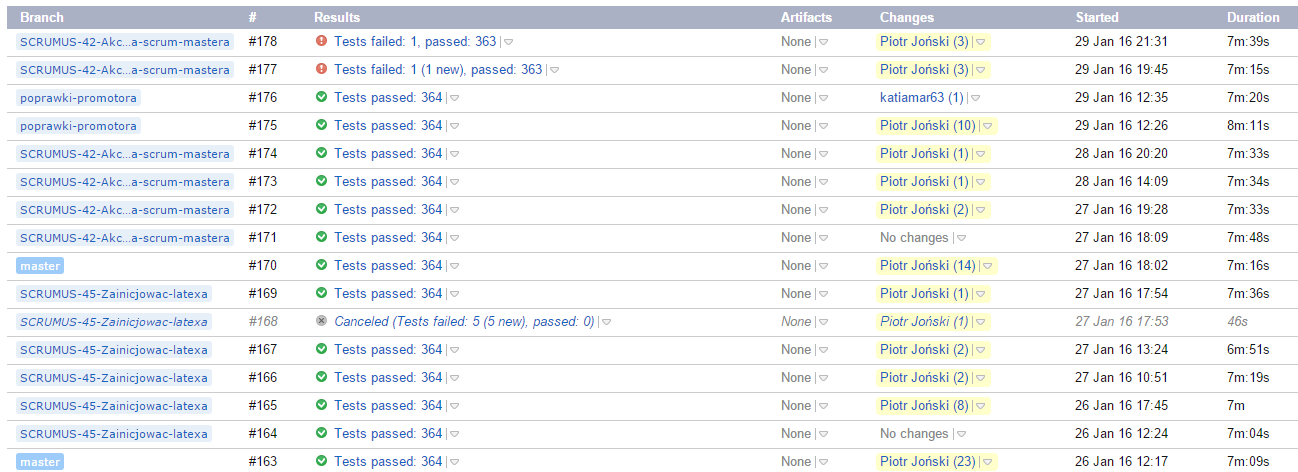
\includegraphics[width=15cm]{rysunki/screenshot_teamcity.png}	
	\caption{Historia budowań projektu w systemie TeamCity}
	\label{fig:teamcity}
\end{figure}


\subsubsection{YouTrack}
YouTrack jest systemem do zarządzania projektami, którego funkcjonalność jest bardzo zbliżona do wcześniej przedstawionego systemu Jira. Jest on dedykowany ogólnie metodykom zwinnym, między innymi Scrumowi. Używałem go podczas implementacji aplikacji, co pozwoliło mi kontrolować zadania, które należy wykonać. Aplikacja umożliwia również generowanie raportów i wykresów dot. zadań, użytkowników czy projektów. System jest również rozwijany przez firmę JetBrains, przez co jest zintegrowany z TeamCity oraz IntelliJ. Pobiera on informacje o budowach projektów z systemu TeamCity oraz umożliwia przeglądania zadań w programie IntelliJ, przez co znacznie upraszcza pracę. Dodatkowo jest darmowy dla małych projektów (do 10 osób), przez co może być wykorzystywany przez małe firmy lub studentów.

\subsubsection{IntelliJ}
IntelliJ jest zintegrowanym środowiskiem deweloperskim na bardzo wysokim poziomie. Umożliwia on tworzenie, kompilację oraz testowanie kodu napisanego w języku Java lub innych językach, które działają na wirtualnej maszynie Javy np. Scala lub Groovy. Narzędzie to posiada szereg funkcjonalności ułatwiających i przyśpieszających programowanie. Jest ono świetnie zintegrowane z frameworkami do testowania (JUnit, Arquillian), systemami do budowania (Gradle, TeamCity), czy zarządzania (YouTrack) przez co programista może się skupić wyłącznie na jednym oknie - oknie aplikacji IntelliJ. Ten system również jest darmowy dla studentów, co stwarza świetne możliwości dla tej grupy osób.


\subsection{Warstwa prezentacji}
Pisząc warstwa prezentacji mam na myśli zarówno część wizualną jak i różne technologie i wzorce pozwalające na budowę własnych aplikacji prezentacji dla istniejącego już systemu. Przy projektowaniu interfejsu WWW pomogły frameworki JSF oraz PrimeFaces, zaś do umożliwienia rozbudowy systemu o dodatkowe aplikacje klienckie odpowiadają przykładowe endpointy w postaci RESTów.

\subsubsection{JSF}
JSF jest frameworkiem, który umożliwia tworzenia warstwy prezentacji dla aplikacji webowych napisanych w języku Java. Posiada on szereg udogodnień, dzięki którym programowanie części wizualnej staje się proste. Framework umożliwia stworzenie warstwy oddzielającej logikę biznesową od widoku, co jest pożądanym, a wręcz wymaganym aspektem programowania aplikacji webowych.

\subsubsection{PrimeFaces}
PrimeFaces jest darmowym frameworkiem, który posiada szereg dostępnych z półki kontrolek służących do obsługiwania widoku. Dodatkowo wprowadza wiele usprawnień, takich jak generowanie tabel z danymi czy szablony css, przez co możemy zmienić wygląd naszej aplikacji za pomocą jednej linii kodu. Został on napisany jako częściowa nakładka na JSF. Wszystkie żądania potrafi obsługiwać synchronicznie i asynchronicznie dzięki zastosowaniu JavaScriptu.

\subsection{Pozostałe}
W tej sekcji zostaną omówione pozostałe aplikacje, frameworki oraz język Java EE.

\subsubsection{Java Enterprise Edition}
Język Java powstał w roku 1995. Jego głównymi założeniami są m.in. niezależność od architektury oraz bezpieczeństwo i niezawodność. Język ten jest dostępny w trzech podstawowych pakietach:
\begin{itemize}
	\item Java Micro Edition - służy do wytwarzania aplikacji na urządzenia, które posiadają niewielkie parametry systemowe. Obecnie wraz z rozwojem telefonów komórkowych i innych urządzeń mobilnych, powstaje coraz mniej aplikacji wykorzystującej ten pakiet.
	\item Java Standard Edition - jest podstawowym pakietem Javy, który można znaleźć na każdym komputerze z zainstalowaną Javą. Oferuje on możliwości programowania sieciowego i współbieżnego. Powstałe aplikacje mogą mieć postać programów uruchamialnych z linii komend lub też pełnoprawnych aplikacji desktopowych.
	\item Java Enterprise Edition - jest to najszerszy pakiet Javy, który oferuje możliwość tworzenia aplikacji webowych z wykorzystaniem różnych technologii takich jak JSF czy EJB. Jest obecnie jednym z najbardziej popularnych narzędzi wykorzystywanych przy implementacji projektów serwerowych.
\end{itemize}

\subsubsection{WildFly}
WildFly jest darmowym kontenerem aplikacji, rozwijanym przez firmę RedHat. Jest on w pełni zgodny ze standardem EJB. Serwer posiada wsparcie dla baz danych oraz zabezpieczeń aplikacji na poziomie kontenerów. Implementuje również specyfikację JAAS (Java Authentication and Authorization Service), dzięki której zapewnione jest bezpieczeństwo w systemie scrumus. Posiada on bardzo dobre parametry takie jak czas startu serwera - poniżej dwóch sekund, czy czas wdrożenia aplikacji - poniżej dziesięciu sekund.

\subsubsection{Docker}
Jest to narzędzie, które w ostatnim czasie zwróciło uwagę wielu firm i indywidualnych programistów. Co prawda koncepcja kontenerów sięga lat 80-tych, jednak dopiero w dobie mikrousług system ten miał możliwość przebicia się. Pozwala on na budowanie obrazów opartych na systemach z rodziny UNIX. Z takich obrazów można tworzyć kontenery, skalować je i zarządzać nimi. System daje możliwość zainstalowania dowolnych aplikacji, przy niewielkiej konfiguracji, co pozwala uruchomić wytworzony w ramach pracy system wraz z bazą danych za pomocą jednej komendy w czasie równym uruchomieniu serwera i wdrożenia aplikacji.

\subsubsection{Postgresql}
Postgresql jest darmową bazą danych o dużych możliwościach. Ma on niewielkie wymagania systemowe oraz oferuje wsparcie dla transakcji. Umożliwia przechowywanie danych o różnych typach i posiada szereg usprawnień optymalizacyjnych. Dodatkowo można definiować własne typy danych.

\subsubsection{\LaTeX}
\LaTeX jest oprogramowaniem do składania tekstu. Posiada szereg funkcjonalności takich jak automatyczne tworzenie spisów treści, tabel czy ilustracji. W łatwy sposób można utworzyć bibliografię i skorowidze. \LaTeX pozwala autorowi odizolować się do wyglądu i formatowania dokumentu, a skupić jedynie na treści i strukturze tekstu. Został on użyty do wytworzenia części opisowej tejże pracy dyplomowej, co znacznie ułatwiło pracę.

\subsubsection{DbSchema}
Jest to program, który pozwala na wizualizację bazy danych oraz zmienianie jej struktury z poziomu programu, bez konieczności wykonywania skryptów SQL. Za pomocą tego programu został wygenerowany model bazy danych przedstawiony w dalszej części tej pracy.

\subsubsection{Lombok}
Framework Lombok służy do automatycznego generowania kodu Javy. Pozwala on za pomocą jednej adnotacji wstawić podstawowe metody do klasy takie jak gettery i settery, konstruktory czy też hashcode i equals. Dzięki temu projektowi nasze klasy zostaną znacznie odchudzone przez co zyskują na czytelności.
